\textbf{7.1.} (1)电阻为 $R$ 的矩形线圈以常速度 $\pmb{v}$ 进入匀强磁场 $B$ 中，见习题7.1(a)图，求线圈中感应电动势和线圈所受的力.

(2) 如果矩形线圈以常速度 $v$ 离开载有稳恒电流 $I$ 的长直导线, 见习题 7.1(b) 图, 求矩形线圈中的感应电动势.


\begin{center}
    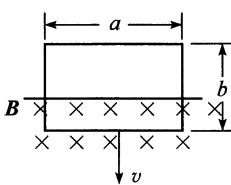
\includegraphics[width=0.3\linewidth]{figures/fig_7_2_1.jpg}
    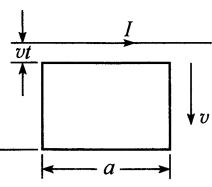
\includegraphics[width=0.3\linewidth]{figures/fig_7_2_2.jpg}
\end{center}

\vfill
\textbf{7.2.} 如习题 7.2 图所示, 一个半径为 $R$ 的圆线圈绕其直径 $PQ$ 以角速度 $\omega$ 匀速转动. 在线圈中心沿 $PQ$ 方向放置一个小磁体, 它的磁矩为 $\mu$ . 试求在点 $P$ 与 $PQ$ 弧中点 $C$ 之间的那段导线上产生的感应电动势.
\begin{center}
    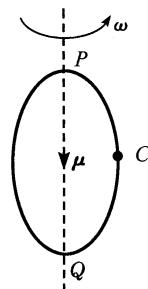
\includegraphics[width=0.15\linewidth]{figures/fig_7_2_3.jpg}
\end{center}


\vfill\newpage

\textbf{7.3.} 如习题 7.3 图所示, 一正三角形线圈的电阻为 R, 边长为 a, 以常角速度 $\omega$ 绕 AB 轴旋转, 均匀磁场 B 与转轴 AB 垂直. 求线圈每两个顶点之间的电势差.
\begin{center}
    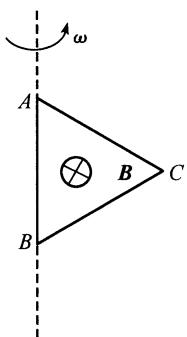
\includegraphics[width=0.15\linewidth]{figures/fig_7_4_1.jpg}
\end{center}
\vfill



\textbf{7.4.} 习题 7.4 图中的轮子由一个半径为 a 的圆环和四根辐条组成, 两个金属刷子分别接触在轮轴和轮边上并与外电阻 R 连接, 外磁场 B 与轴线平行.

(1) 这个轮子产生的感应电动势多大?

(2) 设每根辐条电阻为 r，圆环电阻可以忽略，问 R 取何值时，可获得最大输出功率？

\begin{center}
    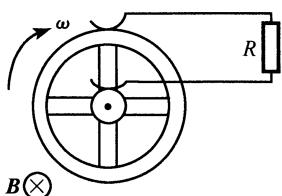
\includegraphics[width=0.25\linewidth]{figures/fig_7_4_2.jpg}
\end{center}

\vfill\newpage

\textbf{7.5.} 一列火车中的一节闷罐车箱宽 $2.5\mathrm{m}$ ，长 $9.5\mathrm{m}$ ，高 $3.5\mathrm{m}$ ，车壁由金属薄板制成。在地球磁场的竖直分量为 $0.62 \times 10^{-4}\mathrm{T}$ 的地方，这个闷罐车以 $60\mathrm{km} \cdot \mathrm{h}^{-1}$ 的速度在水平轨道上向北运动。

(1) 这个闷罐车两边之间的金属板上的感应电动势是多少?

(2) 若考虑车两边积累的电荷所引起的电场,问车内净电场是多少?

(3) 若将两边当作两个非常长的平行平板处理,那么每一边上的面电荷密度是多少?

\vfill



\textbf{7.6.} 一导体盘的半径为 $a$ ，厚度为 $\delta$ ，电导率为 $\sigma$ ，将其放在相对盘轴 $z$ 对称的磁场 $\pmb{B}$ 中
$$
\boldsymbol {B} = B _ {0} (t) \hat {\boldsymbol {z}} \quad (0 \leqslant \rho \leqslant R); \quad \boldsymbol {B} = 0 \quad (\rho > R), \quad R <   a
$$

(1) 确定空间的感应电场；

(2) 确定导体盘的电流密度；

(3) 证明盘耗散的总功率为$\displaystyle P = \frac {\pi \delta \sigma R ^ {4}}{8} \left(\frac {\mathrm{d} B _ {0}}{\mathrm{d} t}\right) ^ {2} \left(1 + 4 \ln \frac {a}{R}\right)$

\vfill\newpage

\textbf{7.7.} 一个大线圈和一个小线圈同心且位于同一平面内，大线圈的半径为 $50\mathrm{cm}$ ，有 $1\times 10^{4}$ 匝，小线圈的面积为 $3\mathrm{cm}^2$ ，有 $5\times 10^{3}$ 匝。

（1）当大线圈中的电流变化率为 $5\times 10^{3}\mathrm{A}\cdot \mathrm{s}^{-1}$ 时，在小线圈中的感应电动势为多少（假定小线圈处的磁场近似均匀）？

（2）如果大线圈载有电流0.2A，且绕它的水平方向的直径以每分钟 $2\times 10^{3}$ 转的速度匀速转动，小线圈在大线圈中心处的水平面上静止，求小线圈中的作为时间函数的感应电动势。

\vfill



\textbf{7.8.} 一环形螺线管有 N 匝, 环半径为 R, 环的横截面为矩形, 其尺寸如习题 7.8 图所示.

(1) 求此螺线管的自感系数；

(2) 求这个环形螺线管和位于它的对称轴处的长直导线之间的互感系数.
\begin{center}
    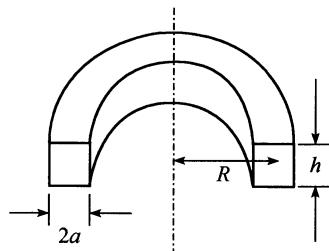
\includegraphics[width=0.3\linewidth]{figures/fig_7_9.jpg}
\end{center}
\vfill\newpage

\textbf{7.9.} 在一个半径为 $10\mathrm{cm}$ 、截面积为 $12\mathrm{cm}^2$ 的圆形铁环上均匀地绕有1200匝绝缘导线，环上有一宽度为 $1\mathrm{mm}$ 的气隙.设铁的相对磁导率是700，它与磁场强度无关，且忽略磁滞效应.

(1) 当有 1A 的电流通过线圈时, 求气隙中的磁场;

(2) 计算该线圈的自感系数.


\vfill



\textbf{7.10.} 一块铜片被弯成如习题7.10图所示形状，已知 $R = 2\mathrm{cm}, l = 10\mathrm{cm}, a = 2\mathrm{cm}, d = 0.4\mathrm{cm}$ ，求

(1) $A, B$ 间管状区的自感系数；

(2) 输入端 $A$ 和输出端 $B$ 之间的电容；

(3) 整个构件的共振频率.
\begin{center}
    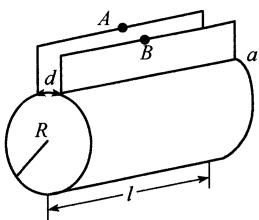
\includegraphics[width=0.3\linewidth]{figures/fig_7_11_2.jpg}
\end{center}
\vfill\newpage

\textbf{7.11.} 一个变压器如习题7.11图所示，线圈 $A, B, C$ 的匝数分别为500, 1000, 500，截面积分别是 $0.005\mathrm{m}^2, 0.001\mathrm{m}^2, 0.0005\mathrm{m}^2$ ，铁芯的水平臂截面积是 $0.002\mathrm{m}^2$ ，如果铁芯的相对磁导率 $\mu_r = 10000$ ，求：

(1) 线圈 A 和 C 间的互感；

(2) 线圈 A 和 B 间的互感.


\begin{center}
    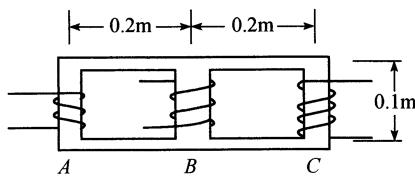
\includegraphics[width=0.35\linewidth]{figures/fig_7_11_3.jpg}
\end{center}

\vfill



\textbf{7.12.} 一电磁铁由 $N$ 匝线圈紧绕在环形轭铁上构成，从轭铁上切去一小段形成气隙，如习题7.12图所示。轭铁环的半径为 $b$ ，环截面的半径为 $a$ ，气隙宽度为 $\omega$ ，铁的磁导率 $\mu$ 为常数。线圈由半径为 $r$ 、电阻率为 $\rho$ 的导线构成，磁铁线圈两端加有电压 $V$ 。为简单起见，假设 $b / a \gg 1, a / r \gg 1, b / w \gg 1$ 。推导下列各量的表达式：

(1) 气隙中的稳定磁场；

(2) 稳态时线圈损耗的功率；

(3) 当电压 V 变化时线圈中电流变化的时间常数.

\begin{center}
    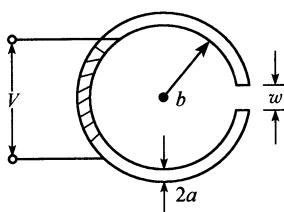
\includegraphics[width=0.3\linewidth]{figures/fig_7_12_1.jpg}
\end{center}

\vfill\newpage


\textbf{7.13} 一个边长分别为 $l$ 和 $\omega$ 的长方形线圈，在 $t = 0$ 时刻正好从如习题7.13图所示的磁场为 $\pmb{B}$ 的区域上方由静止开始向下运动。线圈的电阻为 $R$ ，自感为 $L$ ，质量为 $m$ ，它的上边处在零磁场区。

（1）假定自感可以忽略而电阻不能忽略，求出线圈的作为时间函数的电流和速度；

（2）假定电阻可以忽略而电感不可以忽略，求出线圈的作为时间函数的电流和速度。

\begin{center}
    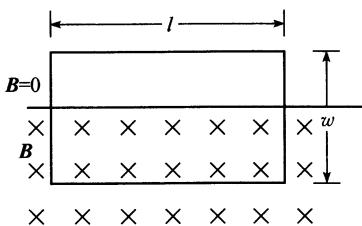
\includegraphics[width=0.3\linewidth]{figures/fig_7_12_2.jpg}
\end{center}

\vfill


\textbf{7.14.} 空心螺线管长 $0.5\mathrm{m}$ , 截面 $1\mathrm{cm}^2$ , 匝数 1000. 忽略边缘效应, 它的自感多大? 一个 100 匝的副线圈也绕在这个螺线管的中部, 互感多大? 现有 1A 的稳恒电流流入副线圈, 螺线管连接着 $10^{3}\Omega$ 的负载. 如果上述稳恒电流突然停止, 将有多少电荷流过电阻?

\vfill

\newpage

\* 7.15 如习题 7.15 图所示, 无电阻的电感器 $L$ 连接金属导轨 $M$ 的一端, 施一恒力 $F$ , 向右拉动金属棒 $N$ . 该棒长为 $l$ , 质量为 $m$ , 在导轨上无摩擦地滑动, 并切割磁力线. 设导轨 $M$ 与金属棒 $N$ 的电阻为零, 棒 $N$ 在水平方向上的初始位置是 $x(0) = 0$ , 初始速度是 $v(0) = 0$ , 那么, 

(1) 电路中电流 $I$ 和坐标 $x$ 之间的关系如何? 

(2) 滑动棒的运动方程是什么? 

(3) 求 $x(t)$;

(4) 试分析滑动棒运动过程中的能量转换过程.
\begin{center}
    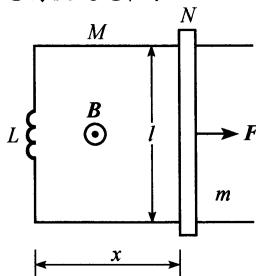
\includegraphics[width=0.25\linewidth]{figures/fig_7_14.jpg}
\end{center}

\vfill



\textbf{7.16.} 由 $3 \times 10^{6} \Omega$ 的电阻、 $1 \mu \mathrm{F}$ 电容和 $\mathcal{E} = 4 \mathrm{~V}$ 的电源连接成简单回路，试求在电路接通后 $1 \mathrm{~s}$ 的时刻，下列各量的变化率：

(1) 电容上电荷增加的速率；

(2) 电容器内储存能量的速率；

(3) 电阻上产生的热功率；

(4) 电源提供的功率.

\vfill\newpage
